\documentclass[12pt, letterpaper]{article}
\usepackage[utf8]{inputenc}
\usepackage[T1]{fontenc}
\usepackage{lmodern}
\usepackage{graphicx}
\usepackage{indentfirst}
\usepackage{geometry}
\usepackage[labelfont=bf]{caption}
\usepackage{wrapfig}
\usepackage{hyperref}
\usepackage[dvipsnames]{xcolor}
\usepackage{enumitem}
\hypersetup{
    colorlinks=true,
    linkcolor=black,
    filecolor=magenta,      
    urlcolor=cyan,
    pdftitle={Overleaf Example},
    }
\usepackage{listings}
\usepackage{xcolor}

\definecolor{codegreen}{rgb}{0,0.6,0}
\definecolor{codegray}{rgb}{0.5,0.5,0.5}
\definecolor{codepurple}{rgb}{0.58,0,0.82}
\definecolor{backcolour}{rgb}{0.95,0.95,0.92}

\lstdefinestyle{mystyle}{
    backgroundcolor=\color{backcolour},   
    commentstyle=\color{codegreen},
    keywordstyle=\color{magenta},
    numberstyle=\tiny\color{codegray},
    stringstyle=\color{codepurple},
    basicstyle=\ttfamily\footnotesize,
    breakatwhitespace=false,         
    breaklines=true,                 
    captionpos=b,                    
    keepspaces=true,                 
    numbers=left,                    
    numbersep=5pt,                  
    showspaces=false,                
    showstringspaces=false,
    showtabs=false,                  
    tabsize=2
}

\lstset{style=mystyle}

\begin{document}
\vspace*{\fill}
\begin{center}
	\includegraphics[scale=0.14]{assets/motorsports_logo.png}
	\includegraphics[scale=0.04]{assets/fav32.png}
	\hspace*{.1in}
	\raisebox{0.21\height}{
\includegraphics[width=0.85\columnwidth]{assets/hgtelemetry.eps}}
	\large{\\[0.5\baselineskip]}
	\large{NYU Baja DAQ Software and Live Telemetry Manual\\[0.4\baselineskip]}
	\normalsize{6/8/2022}
\end{center}
\vspace*{\fill}

\newpage
\tableofcontents
\newpage
\section {Abstract}

In 2020, a small group of graduate computer science students at NYU Tandon was working on a web application project. This system, called Mercury Telemetry, was developed as a theoretical concept for a class in school. At the 2022 Baja SAE Rochester Competition, the NYU Tandon Motorsports team implemented Mercury for the first time and successfully obtained live telemetry. A small box could easily be mounted to track the location, speed, acceleration, direction and many other measurements of the car. All of these measurements could be viewed live by anyone on the team by simply logging on to the website and opening the graphs. Our overall goal of using live telemetry is to improve our performance in the race by catching potential issues in advance if our sensor readings for critical components exceed certain thresholds, thereby also optimizing our lap times, sector times and race strategy.\par However, making this software functional required a lot of effort and reverse-engineering by members of the electronics team from 2021-2022. The current documentation is insufficient to be used as a "quick start guide." Thus, the objective of this manual is to provide detailed instructions for the installation, configuration, use and expansion of NYU Tandon Motorsports' live telemetry system.
\section {Introduction}
In order to understand how the NYU Baja DAQ works, we must analyze the complete data-flow from the sensors obtaining raw data to the ways the user will visualize the final product in the form of graphs, charts, tables, maps and exported files. \textbf{Figure 1} shows this data-flow along with the filenames of the associated code. We chose the Raspberry Pi 4B as our main computer responsible for storing and uploading our sensor data due to its small form factor, low power draw, user-friendliness, APIs and operating system. Upon designing the DAQ, however, the first problem that needed to be addressed was accommodation for both analog and digital sensors. Some analog sensors may include: potentiometers, thermistors, some accelerometers, tachometers,  pressure sensors and voltmeters. Many of these sensors are crucial for improving our understanding of the car during testing; however they are not directly compatible with the Raspberry Pi because it only supports digital IO. Therefore we decided to use Arduino microcontrollers to act as analog to digital converters (ADCs) as well as apply basic calculations using their C-language-based \texttt{.ino} scripts. As seen in \textbf{Figure 1}, these Arduinos directly interface with the Raspberry Pi via a serial USB connection. In other words, we simply connect a long 

\begin{figure}[t]
\centering
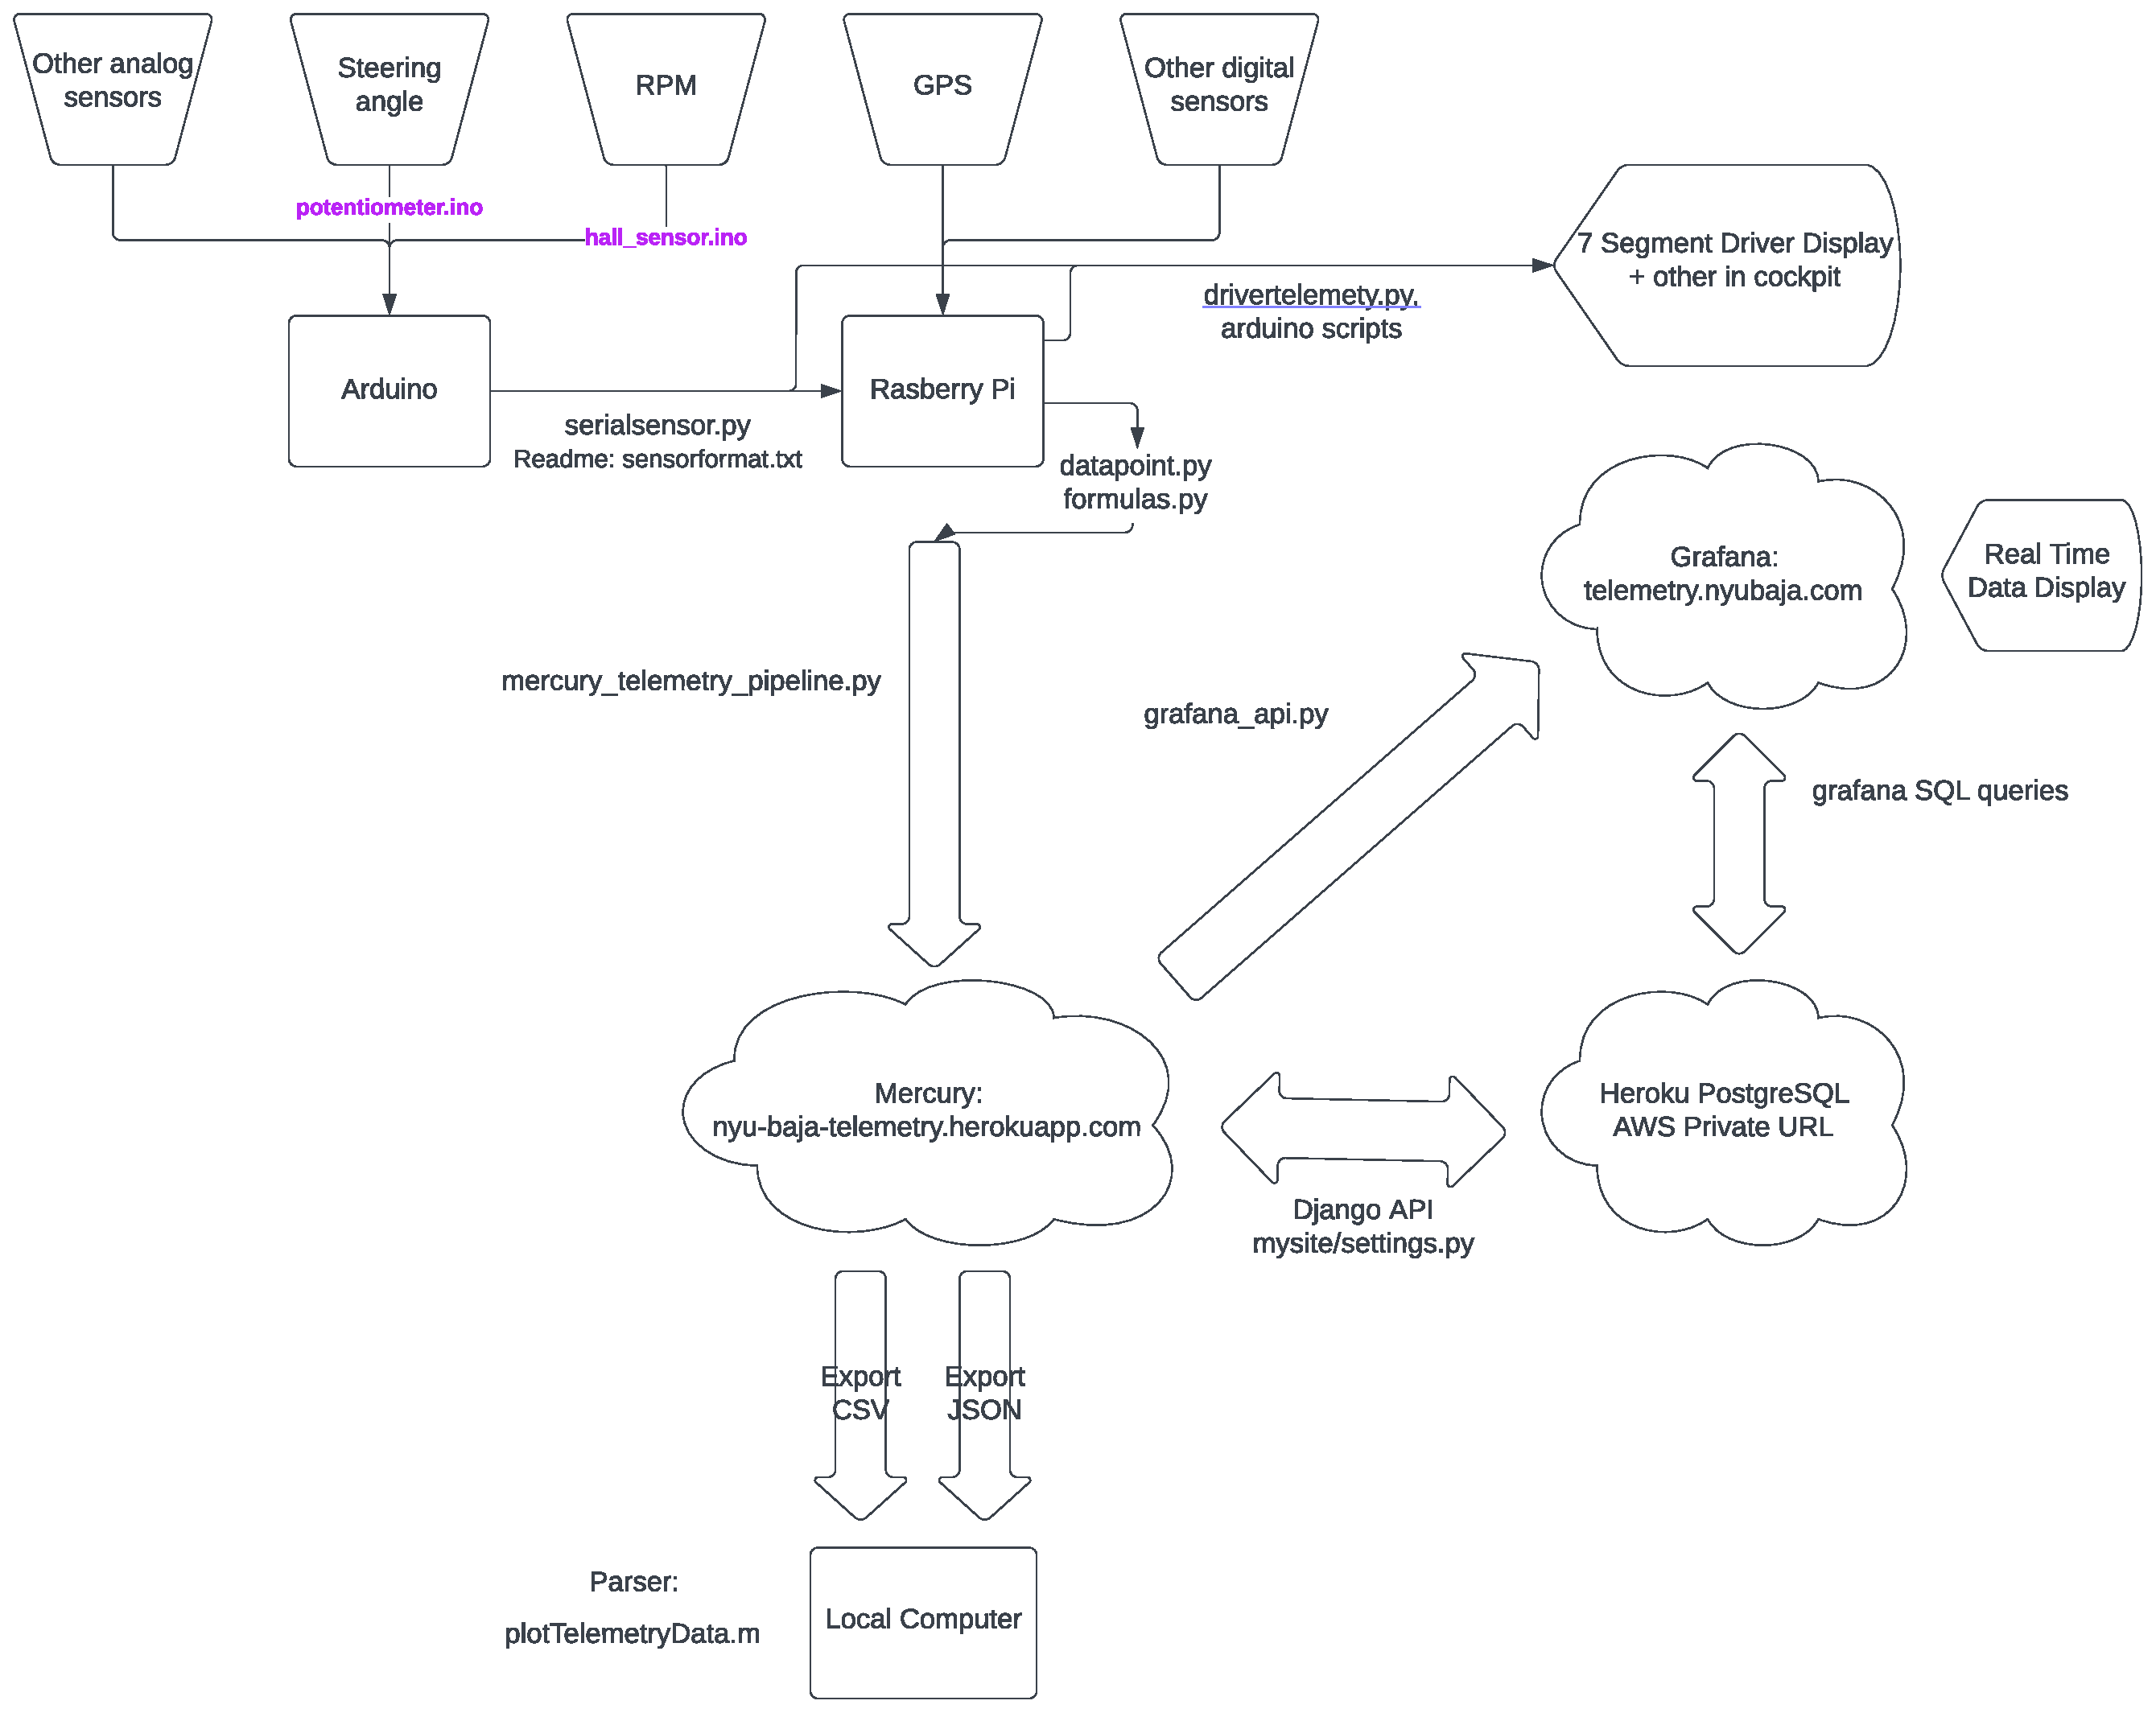
\includegraphics[width=1\columnwidth]{assets/dataflow.eps}
\caption{Flowchart representing overall software dataflow}
\end{figure}



\begin{wrapfigure}[10]{l}{0.5\textwidth}
\includegraphics[scale=0.1]{assets/gpio.png}
\caption{GPIO pinout}
\end{wrapfigure}


{\parfillskip0pt\par}

\noindent USB cable from the Arduino to the Raspberry Pi. To handle digital sensors, we just connect them directly to the Raspberry PI via the GPIO interface seen in \textbf{Figure 2}. There are two dedicated GPIO interfaces called SPI and I2C which utilize specific GPIO pins and these interfaces are often built in to sensors, allowing the user to avoid having to do low level programming.

\par
\newpage




Otherwise we can also just program the GPIO pins directly using the GPIO libraries in Python or whatever language is used to program the Raspberry Pi. Referring back to \textbf{Figure 1}, there is still one very important sensor that needs to be discussed in detail, the GPS and cellular module. The GPS and cellular module is on a special card known as a "hardware at top" board (HAT) which connects to all 40 of the GPIO pins on the Raspberry Pi. Note: even though all 40 pins are connected to the HAT, due to the digital nature of GPIO, pins can still be reused for other purposes. In fact, many HATs can be stacked on top of each other and still function normally. Think of it like a USB hub which splits one port into multiple ports. 

\begin{figure}[h!]
\centering
\includegraphics[width=1\columnwidth]{assets/base-hat-main.jpg}
\caption{Cellular hat and mPCI-E card}
\end{figure}	

	
	\par As seen in \textbf{Figure 3}, the GPS and cellular HAT, manufactured by SIXFAB, is a daughterboard with a mini-PCI-E port which houses a cellular and GPS card made by Quectal. Similar to a Wi-Fi minicard in laptops, this card has 3 mini RF connectors for LTE primary, secondary and GNSS (GPS) antennae. Additionally, the SIXFAB board has a slot for a SIM card which can theoretically work with any major telecommunications provider; however, we chose to use the SIXFAB SIM card because as a part of the SIXFAB ecosystem, the card is integrated to an online portal which allows for easy installation and configuration of the system. Additionally, SIXFAB even has a remote terminal allowing the user to control the Raspberry Pi via the command line from anywhere as long as it is powered on and has cellular service. In addition to giving us remote control of the Raspberry Pi, the cellular module will be the  main means of communication between the Raspberry Pi and Mercury Telemetry. 
	\par Before we introduce Mercury Telemetry, we must briefly note the driver telemetry, the motivation of which is to provide important metrics for the driver to see while the car is running. Just as we can read sensor data via serial, I2C, SPI and GPIO connections, we can write data as well. With that in mind, we designed a function class called \texttt{drivertelemetry.py} to have functions that can be called to send values to output devices such as a 7 segment display to be viewed by the driver. Speed, lap times, sector times and messages from the paddock are currently under consideration for implementation.
	\par 
	Now we will introduce Mercury Telemetry. Mercury Telemetry is a web application which manages a sequel (SQL) database which is essentially a large queryable data structure with tables holding information for the website, organizing the sensor measurements and the sensor data itself. This project is an open source, general purpose telemetry application intended for university and amateur vehicle competition teams. Mercury Telemetry can be used to collect remote measurements from competition vehicles, then relay and display them to inform the vehicle's crew of key status indicators.

	Collection of basic, generally useful data points like speed, acceleration, orientation, and GPS location will be covered in the project. If other data points not covered in this project would be useful for a vehicle team, Mercury Telemetry's modular design is intended to be easy to modify to fit new data collection use cases.
	\textbf{Figure 4} shows the overall structure of the SQL database for Mercury. It may seem large and complicated, but we can consider each box step by step and we don't need to worry about the majority of what's there. The database is logically structured  based on how the information needs to be organized. Mercury is organized in terms of events. Think of an event as a data acquisition session that should be separated on its own. Each event has a venue and a set of measurements. In \textbf{Figure 4}, let's look first at \texttt{ag\char`_data\char`_agmeasurement}. The structure contains a UUID, timestamp, value, event UUID, and sensor ID. The UUIDs for both the event and the measurement are called "universally unique identifiers" and are used as references for when the database needs to be queried. For example, if we needed to find how fast the car was going at a certain time, the program would find what the UUID of the sensor for speed is and then obtain the value. We must also note the datatype of the measurement's value which is a JSON. The JSON is a neat datatype because it is a set of nested \textbf{maps} represented by a string delimited by curly brackets. JSON models can represent data of an arbitrary size so it is extremely powerful. \\[3\baselineskip]
	The JSON model for measurements are in the following format:
	
\begin{verbatim}
{
    "sensor_id": << sensor id number >>,
    "values": {
        "value_x" : << some value >>,
        "value_y" : << some value >>,
        "value_z" : << some value >>
    }
    "date" : << ISO 8601 date/time >>
}
\end{verbatim}


	
\begin{figure}[t!]
\centering
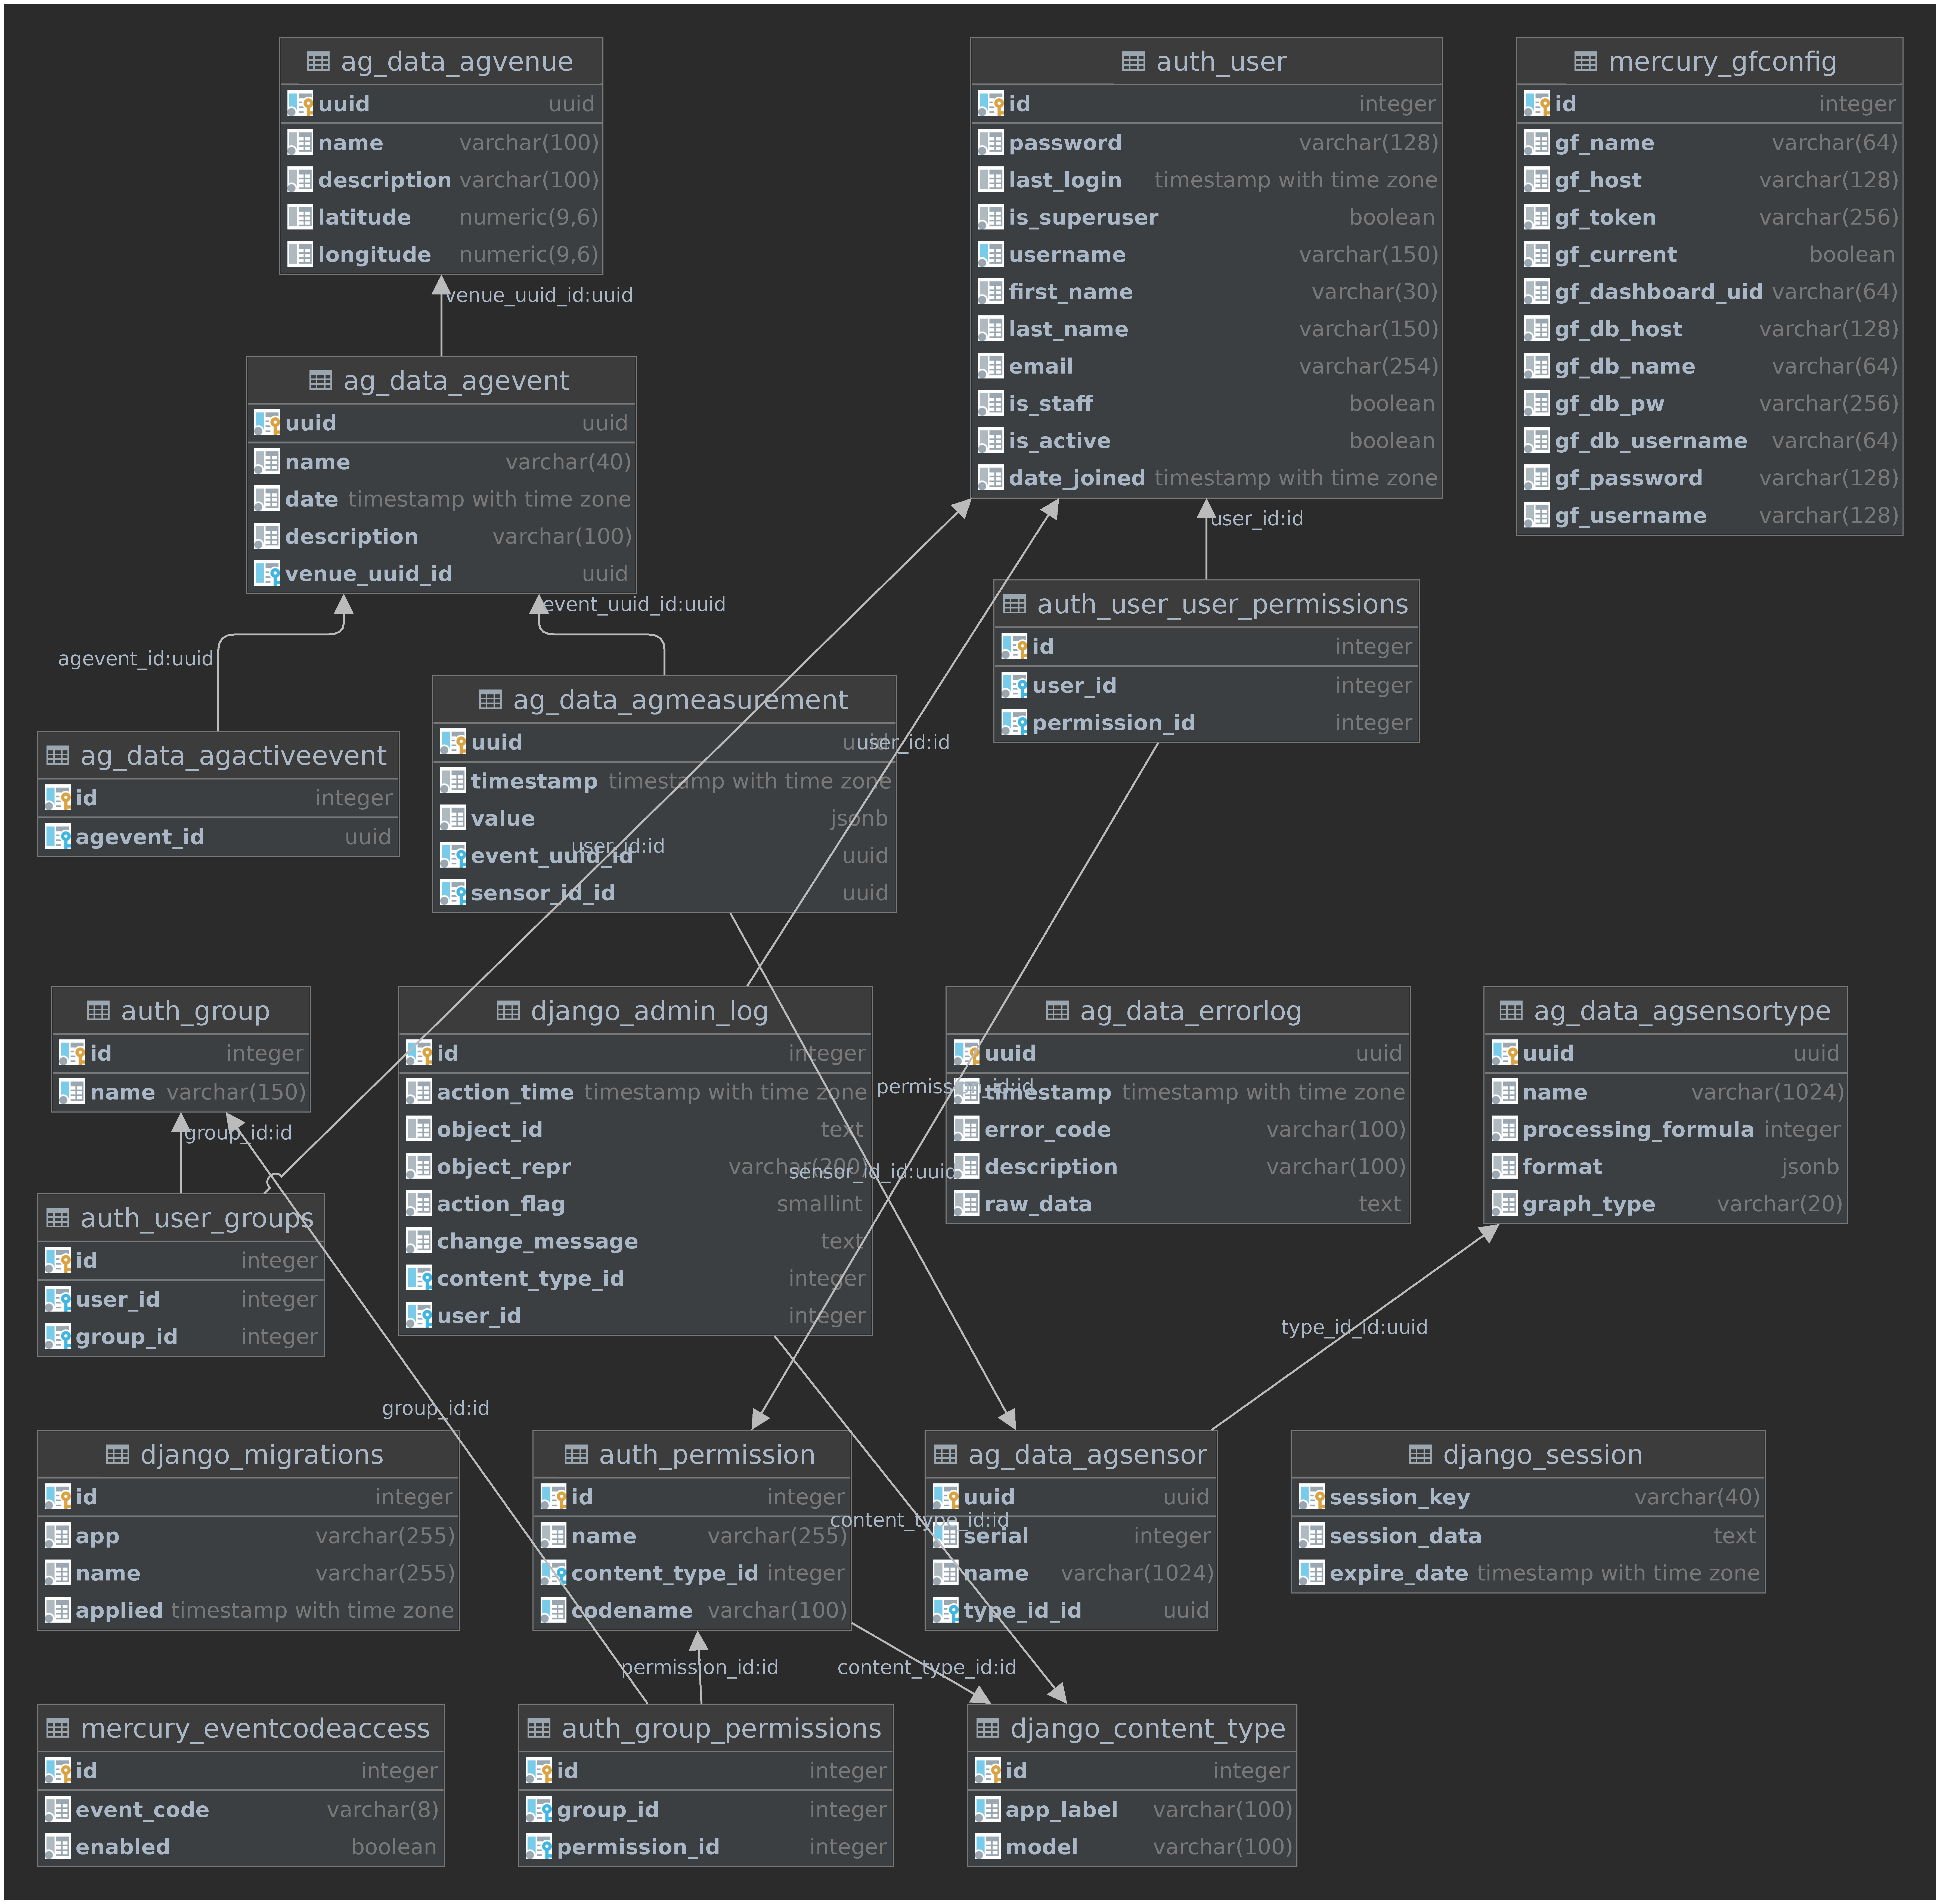
\includegraphics[width=1\columnwidth]{assets/Mercury-Database.eps}
\caption{Mercury's SQL Database Structure generated by DataGrip}
\end{figure}	 

\par As seen in the following code, the JSON structure of each sensor measurement contains the ID, values and date. What is stored in the \texttt{"value"} field in the \texttt{ag\char`_data\char`_agmeasurement} box
is only the nested JSON within the \texttt{"values"} key. The full JSON represents what is actually uploaded to the website through POST requests. Later in the manual, we will discuss in detail the process for sending POST requests to Mercury. Looking at the contents of \texttt{"values"}, we see \texttt{"value\char`_x"}, \texttt{"value\char`_y"}, and \texttt{"value\char`_z"}. The names of the keys in this example are arbitrary and can be anything based on what the user decides on the website. Moreover, the number of values is unlimited. For instance, a gyroscope sensor reading may have a value field as:

\begin{verbatim}
{
   "yaw" : 3.2234,
   "pitch" : 8.9009,
   "roll" :  0.2792
}
\end{verbatim}
 
\par Now that we understand how sensor data is stored in the SQL database, we can consider how these measurements are organized. Referring back to \textbf{Figure 4}, \texttt{ag\char`_data\char`_agmeasurement} points to \texttt{ag\char`_data\char`_agsensor} which itself points to \\ \texttt{ag\char`_data\char`_agsensortype}. These two structures contain information on the type of data the sensor uses and the graph that will be used by default on Grafana. We need to know whether a sensor will be using a graph, gauge or map and for its datatype: numbers, strings or bools. Additionally, \texttt{ag\char`_data\char`_agmeasurement} points to \texttt{ag\char`_data\char`_agevent} which itself points to \texttt{ag\char`_data\char`_agvenue}. As mentioned previously, measurements are organized by events. These events contain names, descriptions and dates. The events also require a "venue" which also has its own fields including the name, description and location. As of right now, the "venue" structure does not have any functionality other than having fields.

\par Some of the boxes we do not have to worry too much about are the ones beginning with \texttt{django} and \texttt{auth}. These structures are pertinent to logging into and managing the hosted website. Django is the Python API used to make websites which revolve around an SQL database. \texttt{mercury\char`_eventcodeaccess} holds the secret passcode to access the website. 
	
	\par The last box we need to discuss is \texttt{mercury\char`_gfconfig}. This contains all of the fields necessary for Mercury to interface with Grafana. In order to control Grafana, Mercury stores Grafana's API key and sends POST requests to Grafana in order to invoke its commands. 
	\par Before we discuss how Mercury manages Grafana, let's first talk about what Grafana actually is. Grafana is an engine which queries online databases at regular intervals and uses those queries to generate live graphs. Below is a sample SQL query used by Grafana.

\begin{figure}[t!]
\centering
\includegraphics[width=1\columnwidth]{assets/grafana-example.png}
\caption{Sample Grafana dashboard from 2022 Baja SAE Rochester}
\end{figure}	
	
\begin{verbatim}
    SELECT "timestamp" AS "time",
    CAST(value->'result'->'speed' AS float) AS "speed"
    FROM ag_data_agmeasurement
    WHERE $__timeFilter("timestamp") AND sensor_id_id='7b1e9529-522c-42df
    -a922-9694f9c32cc7'
    AND "event_uuid_id"='935d7301-a707-4e98-b72b-3a6a823d29c6'
    ORDER BY timestamp
\end{verbatim}
	
	 The above code is constantly being executed to get the tables to generate each graph. In the case of Mercury, there is an SQL database with measurements being regularly appended to it. Each time a measurement is added, Grafana updates the graph accordingly. Mercury actually makes our lives easier by automatically generating the SQL queries for Grafana depending on the sensor type similar to the above so we do not have to manually code them. \textbf{Figure 5} is what the user would see while viewing a Grafana dashboard. On the top left is the name of the dashboard which corresponds to the name of the event in Mercury. On the dashboard itself there are three live graphs. On the top left is a normal line graph which was used to show the speed of the GPS sensor. On the top right is a log which was set as a table that accepted string data. Finally on bottom left is the TrackMap. This "panel" (as it is known within the context of Grafana) is actually an external plugin. Since Grafana is open-source, there are tons of modifications and extensions for it. The TrackMap traces routes from GPS coordinate data.
	 
\par This was an introduction on how NYU Baja's DAQ system works. If you are still unsure on the organization of the system, please refer back to \textbf{Figure 1} for the flow of data. For instructions on how to set up and get started, please continue reading ahead.
	

	




\section {Programming Prerequisites and Developing Environment}
\par All members working on the NYU Baja DAQ Software should be familiar with the following: 
\begin{itemize}
	\item Git / Github
	\item Bash
	\item Linux
	\item \texttt{.sh} scripts
	\item Python
	\item Python virtual environments and \texttt{requirements.txt}
	\item \texttt{pip}
	\item C
	\item Arduino (programming language)
	\item Docker (optional but preferred)
\end{itemize}
\par If you are unsure of any of the aforementioned items, feel free to ask other teammates to find out how it works. The amount of knowledge required depends on whether you are just using the telemetry or actually adding additional functionality to it. Regardless, it is crucial to have an understanding of Git, Bash, Linux and Pip as they are required for installation. \\

Below is a basic git tutorial. If you would like more detailed documentation, please visit the following \href{https://docs.google.com/document/d/1UZTql9ehKAVS1FU45GWRngsuxctNcDY6T-cq5tJqQJY/edit?usp=sharing}{link}. Note: YOU NEED TO BE A MEMBER OF THE BAJA DRIVE IN ORDER TO ACCESS THIS DOCUMENT.  \\[1\baselineskip]

\noindent Git Bash Installation: \\[1\baselineskip]

\noindent\url{https://git-scm.com/downloads} \\[1\baselineskip]

\noindent On Mac OS, you can either run the installer or use the homebrew package manager to install git from the command line. \\[1\baselineskip]

\noindent{\texttt{\$ brew install git} \\[1\baselineskip]}

\noindent On Windows, download the \texttt{.exe} and run the wizard. In installation options, you can use either the git bash or the Windows command prompt. If you elect to use the Windows command prompt, then some of your commands will differ for moving around the file structure. \\[1\baselineskip]

\noindent On Linux, or WSL, use the distro’s package manager to install git. \\[1\baselineskip]

\noindent For Debian based distributions:\\[1\baselineskip]

\noindent{\texttt{\$ sudo apt update}} \\
\texttt{\$ sudo apt install git} \\[1\baselineskip]

\noindent For other distributions: \\[1\baselineskip]

\noindent See \url{https://git-scm.com/download/linux}. \\[1\baselineskip]


Useful Git and Bash Commands:
\begin{itemize}
	\item \texttt{cd} = change directory
	\begin{itemize}
		\item Move around file structure
		\item \texttt{cd ..} goes backwards one directory
	\end{itemize}
	\item \texttt{touch ‘filename.extension’} (\texttt{type >> nul ‘filename.extension’} in Windows cmd)
	\begin{itemize}
		\item Creates a new file in the current directory
		\item Placing a . before the filename will create a hidden file\\
		(i.e. ‘touch .example.py’ will create a hidden python file
	\end{itemize}
	\item \texttt{mkdir} ‘directory name’
	\begin{itemize}
		\item makes new folder
	\end{itemize}
	\item \texttt{ls} = list (\texttt{dir} in cmd)
	\begin{itemize}
		\item See what files and folders are available to cd into in your working directory
	\end{itemize}
	\item \texttt{ls -a} (\texttt{dir /a} in cmd)
	\begin{itemize}
		\item Displays all files and folders available in directory (also shows hidden files such as the file created from ‘git init’)
	\end{itemize}
	\item \texttt{git init} (only use this command to create new repositories)
	\begin{itemize}
		\item Initializes github repository, from now on repository will be shortened as repo
	\end{itemize}
	\item \texttt{git add .}
	\begin{itemize}
		\item Adds all changes to staging area (except .gitignore see section on .gitignore)
		\item Use git add *filename* to add a single file to the staging area
	\end{itemize}
	\item \texttt{git commit -m “comment”}
	\begin{itemize}
		\item Commits changes and adds comment
	\end{itemize}
	\item \texttt{git push}
	\begin{itemize}
		\item Pushes changes to github
		\item When pushing, it is good practice to alert your teammates of any major changes that get pushed.
		\item For working projects, DO NOT push broken code. Your teammates do not want to pull and find out the code will not compile/run. 
	\end{itemize}
	\item \texttt{git clone} *url of repo*
		\begin{itemize}
			\item Creates local copy of repository 
			\item \textbf{Local} means on your computer, not in the cloud
			\item \textbf{Remote} refers what’s in the cloud (online)
		\end{itemize}
	\item \texttt{git pull}
		\begin{itemize}
			\item Updates the current working directory with the code online.
			\item If you make changes to the working directory and then pull, a merge will occur.
			\item If your changes were made in different sections than the code online, then the merge will be automatic. Otherwise you will need to manually fix merge conflicts. 
			\end{itemize} 
			\item \texttt{.gitignore}
			\begin{itemize}
				\item Is a file which tells github to ignore certain files and directories when using “git add .”
				\item Many directories and binaries may be IDE specific or could contain system specific libraries / configurations. We do not want those on github. What is on github should work on any system the repo is designed for.
			\end{itemize}
\end{itemize}

\par One more software prerequisite we must consider is \texttt{pip} (package installer for Python) and \texttt{venv} (Python virtual environments). When programming, we often need to use external libraries for additional functionality by importing that class/file. In Python, not all of the libraries are installed by default; therefore, it is sometimes necessary to use \texttt{pip} to enable that functionality. For example in order to send a POST request (necessary for sending measurements to Mercury), we need to install the \texttt{requests} library. This installation can be done simply by executing the following command in Bash: \\[1\baselineskip]\

\texttt{pip3 install requests} \\[1\baselineskip]

\noindent Note: we need to say \texttt{pip3} because we are using Python version 3 or greater. \\

\par However this presents a problem. Python was made to be a lightweight language. It should not be the client's job to make sure their Python libraries are up to date with all of the Python programs that they are using. What is the point of having to load Python with 100+ libraries installed, when you are just doing a \texttt{"hello world"}? The answer is that would be extremely poor practice. 

\par Python has created a mitigation for this issue with the \textbf{virtual environment}. A virtual environment contains its own separate Python runtime executables and is specific to the project you are working on. Think of it like a clone of Python, but designed specifically for your project. The implication of having project-specific executables is that you would also have \textbf{project-specific libraries}. This means each project gets only the libraries they need to run, eliminating compatibility complications and maximizing speed. 

\par How does one know a project requires a virtual environment? The answer is in the text file \texttt{requirements.txt}. \texttt{requirements.txt} is a plain text file listing the required libraries and their versions a Python project needs. For more info on \texttt{requirements.txt}, see \url{https://pip.pypa.io/en/stable/user_guide/}. Below is an example of the requirements for the Basic DAQ Software. 

\begin{verbatim}
	requests==2.28.1 #means that it will only install 2.28.1
	RPi.GPIO>=0.7 #means the latest version greater than 0.7
	adafruit-blinka
	adafruit-circuitpython-max31855
	adafruit-circuitpython-lis3dh
	adafruit-circuitpython-l3gd20
	numpy
	raspberrypi-tm1637
	keyboard
\end{verbatim}

\par As seen in the text above, the requirements for Basic DAQ Software are mostly libraries for the Raspberry PI and sensors allowing for less low-level coding. All the user needs to do to start developing is install a virtual environment and the requirements. To use venv go to \url{https://docs.python.org/3/library/venv.html} or follow these steps: \\[1\baselineskip]

\noindent cd into the project directory then execute: \\
\texttt{python3 -m venv venv}.\\[1\baselineskip]

\noindent cd into \texttt{venv\textbackslash bin} then execute:
\texttt{source activate}. The virtual environment has been activated \\[1\baselineskip]

\noindent Now we can install the requirements. Python has a specific command which installs all of the required libraries at the same time using \texttt{requirements.txt}: \\[1\baselineskip]

\texttt{pip3 install -r requirements.txt} \\[1\baselineskip]


\par In terms of the developing environment, we will review which OS is required to test the code for the NYU Tandon DAQ Software. For the Basic DAQ Software, a Raspberry PI 4B running Raspbian is required. Since Raspbian is a Debian-based distribution, the code would also work in a regular Ubuntu machine; however any Raspberry-PI specific code needs to be disabled (more on that later). 

\par For Mercury Telemetry, it is \textbf{strongly} recommended to use a \textbf{Debian-based} distribution of \textbf{Linux} such as \textbf{Ubuntu}. WSL (Windows Subsystem for Linux) has also been proven to work but be prepared to spend some time and effort setting it up. A tutorial for WSL can be found at \url{https://docs.microsoft.com/en-us/windows/wsl/}. With a good understanding of git, venv, pip and bash, you will be able to install and run NYU's DAQ software. The instructions provided in the sections below will show the user how to run the NYU Baja DAQ system.


\section {Hardware Setup}

\par The minimum hardware requirements are as follows: 

\begin{itemize}
	\item Raspberry Pi 4B
	\item USB C power @ 5.1V. The power supply must be capable of 3A when the Pi is under load. We strongly recommend adding a switch for the DAQ that the driver can reach.
	\begin{itemize}
		\item NOTE: On custom power delivery solutions, you might need to increase the voltage to as high as 5.75V to avoid low voltage warnings. That is fine. The Raspberry Pi has a built-in active voltage regulator. If you get a high voltage warning then decrease the supply voltage until there are no more warnings.
		\item NOTE: The Raspberry Pi is a computer, which means it has a variable power draw and thus a variable current draw. For that reason, you MUST use \textbf{active} voltage regulation such as a \textbf{buck converter} OR a battery with the exact specified voltage. \textbf{DO NOT try using a series resistor to regulate the voltage of the Raspberry Pi.}
	\end{itemize}
	\item SIXFAB Raspberry PI Base Hat with pins
	\item Cellular / GPS PCIE minicard (Quectal or Telit must be sold by SIXFAB to work) 
	\item SIXFAB SIM Card
	\item Short micro USB to USB type A connector
	\item Micro HDMI to HDMI connector
	\item 3 RF antennae (that can connect to WiFi minicard antennae size)
	\item Standoffs, washers and screws (for Raspberry Pi HATs)
	\item \textbf{Fully waterproof case that can also disapate the heat of the Raspberry Pi.} This is a major design goal that should be prioritized.
	\begin{itemize}
		\item Obviously, the system will still work fine without the case but as soon as it is going to be used on the car, waterproofing precautions must be taken. This is especially true for competition-style tracks which are VERY muddy.
	\end{itemize}
	
\end{itemize}
 
\par Below are the instructions on how to assemble the Raspberry Pi and SIXFAB HAT:

\begin{enumerate}[label=\large{\textbf{\arabic*}.}]
	\item \textbf{\large{Attach the Quectel EC25/EG25 mini PCIe module to the HAT.}}
	\begin{figure}[h!]
	\centering
	\includegraphics[width=1\columnwidth]{assets/Raspberry-Pi-Base-HAT-Quectel-Getting-Started-1-scaled.jpg}
	\caption{Placement of mPCIE module}
	\end{figure}	
	\item \textbf{\large{Attach the antenna to the mini PCIe module.}}
	\begin{itemize}
	\item Make sure the right antenna is connected to the right port. Attach LTE full band PCB antenna/LTE connector of the LTE-GNSS dual antenna to the main Antenna interface/diversity antenna interface and GPS Antenna portion goes to the GNSS antenna interface.
	\begin{figure}[h!]
	\centering
	\includegraphics[width=1\columnwidth]{assets/e4f78fd-EC25_Antenna_ports-848x300.jpg}
	\caption{EC25 Antenna interface}
	\end{figure}	
	\begin{figure}[h!]
	\centering
	\includegraphics[width=1\columnwidth]{assets/Raspberry-Pi-Base-HAT-Quectel-Getting-Started-2-scaled.jpg}
	\caption{GPS antennae connection}
	\end{figure}	
	
	\end{itemize}
	\item \textbf{\large{Attach 40 pin header to the Base HAT that comes with the HAT and insert the Sixfab Connect SIM to Base HAT.}}
	\begin{figure}[h!]
	\centering
	\includegraphics[width=1\columnwidth]{assets/Raspberry-Pi-Base-HAT-Quectel-Getting-Started-3-scaled.jpg}
	\caption{40 pin header connection}
	\end{figure}
	\newpage	
	\item \textbf{\large{Now attach the HAT to the Raspberry Pi.}}
	\begin{figure}[h!]
	\centering
	\includegraphics[width=1\columnwidth]{assets/Raspberry-Pi-Base-HAT-Quectel-Getting-Started-4-scaled.jpg}
	\caption{Nearly done Hardware Setup}
	\end{figure}	
	\newpage
	\item \textbf{\large{Finally connect the micro-USB cable to the HAT and Raspberry Pi.}}
	\begin{figure}[h!]
	\centering
	\includegraphics[width=1\columnwidth]{assets/Raspberry-Pi-Base-HAT-Quectel-Getting-Started-5-scaled.jpg}
	\caption{Full Hardware Setup}
	\end{figure}	
\end{enumerate}


\section {Raspberry Pi and GPS Configuration}

\par Raspberry Pi(s) are designed to run a Linux distribution called Raspberry Pi OS. It lives on the Raspberry Pi's main storage which happens to be a Micro-SD card. To install the Raspberry Pi OS on the Raspberry Pi, go to the following website: \\
\par{\url{https://www.raspberrypi.com/software/}}\\
\par Download the Raspberry Pi OS imager tool and follow the instructions in the wizard to load the OS on the SD card. Once the SD card is attached,  connect the Raspberry Pi to a Micro-HDMI cable and attach that to a display. Additionally, connect a keyboard and mouse and boot the Raspberry Pi by connecting the USB C power supply. \\

\noindent{\textbf{\large{Setting up Raspberry Pi OS:}} \\

\par When the Raspberry Pi boots up for the first time, follow the on-screen instructions and enter the basic configuration. After a username and password is chosen, you will be prompted to update the OS. Once the update is complete, you can use the Raspberry Pi. \\

\noindent{\textbf{\large{Setting up the SIXFAB software: (from SIXFAB WEBSITE)}} \\

\par We have completed the hardware setup, now we will install SIXFAB CORE for a smooth and reliable cellular connection. The SIXFAB CORE contains the device drivers for the HAT, SIM card and GPS module.

\begin{enumerate}[label=\large{\textbf{\arabic*}.}]
	\item \textbf{\large{Create SIXFAB Account}} \\[1\baselineskip]
	\noindent Go to \url{https://connect.sixfab.com}, create an account and log in.
	\item \textbf{\large{Register your first SIM and Add Coupon/Credit}} \\[1\baselineskip]
	If you are logging into Connect for the first time, follow the 			
	'Quickstart' steps first. If not, continue with step 3.
	Register your SIM with its ICCID and giving it a name. Add your credit 
	card or add credit using the \$25 coupon code provided by Sixfab that 
	comes with the kit.
	\item \textbf{\large{Register a SIM}} \\[1\baselineskip]
	\noindent Register and activate a SIM from the \textbf{"SIM -> Register a SIM"} section. Skip this step if you already have an active registered SIM.
	\item \textbf{\large{Create Device}} \\[1\baselineskip]
	\noindent Now everything is ready to install Sixfab CORE on the device.
An active Sixfab SIM is required to create a device. Activate the SIM from the SIM details page. \\[0.5\baselineskip]
	\noindent View your available SIM cards by going to \textbf{"SIM -> My SIMs"}. Click on the \textbf{"Create Device"} link in the row the SIM for which you will create the device.
	\item \textbf{\large{Select Region and Board for Device}} \\[1\baselineskip]	
	\noindent We are using Global, Raspberry Pi.
	\item \textbf{\large{Copy Installation Code}} \\[1\baselineskip]
	\begin{figure}[h!]
	\centering
	\includegraphics[width=1\columnwidth]{assets/Sixfab-Connect-SIM-Data-Management-select-region.png}
	\caption{Device and Region selection and Unique installation code}
	\end{figure}	
	\item \textbf{\large{Keep the USB Cable unplugged from the HAT}} \\[1\baselineskip]
	\noindent If the USB cable is plugged in, unplug the USB.
	\item \textbf{\large{Run the installation script}} \\[1\baselineskip]
	Open a terminal on the Raspberry Pi and run the installation code you have just copied. The following output should be seen in the terminal.
	\begin{verbatim}
	pi@raspberrypi:~ $ sudo bash -c "$(curl -sN 
	https://install.connect.sixfab.com)" -- -t 
	YOUR_TOKEN_APPEARS_HERE' -d
    .&@&.             %%          .%@%           
   #@@@%           *&@@@&.         %@@@#         
  &@@&. .&@@%   .%@@@@@%/.   .%@@&. ,&@@%        
 %@@&. /@@@#  *&@@@@&&&@@@@&,  %@@&* .&@@&       
/@@@* .@@@#  &@@&(       (@@@%  #@@&, *@@@*      
%@@&. #@@&. (@@@,         ,&@@( .@@@(  &@@#      
%@@&. #@@&. /@@@,         *&@@( .@@@(  &@@#      
*@@@* .&@@#  %@@@#       %@@@#  #@@&, /@@@,      
 %@@&, *@@@%  .&@@@@@@@@@@@%. .&@@&, ,&@@%       
  %@@&*  %@@#     *#%%%#*     #@@%  *&@@%        
   (@@@&.                         .&@@&/         
     #@#                           #@#    

  ____  _       __       _        ____               
 / ___|(_)_  __/ _| __ _| |__    / ___|___  _ __ ___ 
 \___ \| \ \/ / |_ / _` | '_ \  | |   / _ \| '__/ _ \
  ___) | |>  <|  _| (_| | |_) | | |__| (_) | | |  __/
 |____/|_/_/\_\_|  \__,_|_.__/   \____\___/|_|  \___|
=====================================================
[INFO]  Creating sixfab user...
[INFO]  Updating sudoers...
[INFO]  Sudoers updated
[INFO]  Updating system package index...
[INFO]  Looking for dependencies...
[INFO]  Git is not installed, installing...
[INFO]  Pip for python3 is not installed, installing...
[INFO]  ifmetric is not installed, installing...
[INFO]  Installing Sixfab ATCom tool...
[INFO]  Sixfab ATCom installed
[INFO]  Initializing environment file...
[INFO]  Initialized environment file
[INFO]  Downloading agent source...
[INFO]  Installing agent dependencies...
[INFO]  Installed agent dependencies.
[INFO]  Initializing agent service...
[INFO]  Agent service initialized successfully.
[INFO]  Downloading manager source...
[INFO]  Installing manager dependencies...
[INFO]  Installed manager dependencies.
[INFO]  Initializing manager service...
[INFO]  Manager service initialized successfully.
[INFO]  Setting default network priority : eth0 > wlan0 > usb0 = wwan0
[DONE]  Installation completed successfully.

-----------------------------------------------------------------------
Press ENTER to reboot your system. (Recommended)
Press Ctrl+C (^C) to finish installation without reboot.

Reminder: Plug the USB cable to Sixfab HAT!
Warning: Network priority settings will be effective after reboot!
-----------------------------------------------------------------------
	\end{verbatim}
	\item \textbf{\large{Plug the USB Cable to the HAT}} \\[1\baselineskip]
	\noindent Once the installation is completed successfully, Hit Enter to reboot the Raspberry Pi and plug the USB cable to the HAT.
	\item \textbf{\large{Installation Complete}} \\[1\baselineskip]
	\noindent Refresh the device page after the installation is complete. The following dashboard will appear with the device information. After a successful connection, please wait for 3-5 minutes for the data to appear on the dashboard.
	\begin{figure}[h!]
	\centering
	\includegraphics[width=1\columnwidth]{assets/Sixfab-Connect-SIM-Data-Management-getting-started-modem-kit.png}
	\caption{SIXFAB Dashboard once device installation is complete}
	\end{figure}	
	\newpage \noindent The dashboard shows the device online status, how much data is used, and which connection method is currently being utilized (wifi vs cellular). Additionally, the dashboard has a remote terminal which we will be using at competition and later in the tutorial.
\end{enumerate}

\par Now that the driver has been installed for the cellular HAT, we should now have a 4G LTE internet connection for the Raspberry Pi. Check to make sure internet access works by disconnecting from Wi-Fi. You should be able to see a icon appear on the top right of the taskbar in Raspberry Pi OS for the network selection toolbar. Additionally, there should be blinking red and blue LEDs on the HAT indicating that it is working properly. 

\par We can now install the GPS test software. We will be using two popular open-source tools for testing GPS modules, GPSD (GPS Daemon) and GPSMon (GPS Monitor). These command-line tools interface with GPS hardware which communicates to the Pi via  serial using a standard syntax called NMEA 0183 sentences. These sentences contain all of the data the GPS collects such as the positioning of the satellites it finds, whether the GPS has an accurate fix and all of the derived measurements such as position, speed, heading, etc. Additionally, we wrote a script which initializes the SIXFAB GPS, starts the daemon and launches GPSMon. GPSmon will help us check to make sure the GPS is working before we use it for TrackMap. 

\par First, let's install the Linux GPS tools. In terminal type the following: \\[1\baselineskip]

\par{\texttt{sudo apt-get install gpsd gpsd-clients python-gps}}\\[1\baselineskip]
\par Next make sure \texttt{Basic\char`_DAQ\char`_Software} is cloned on the Raspberry Pi.  Cd into the \texttt{testgps} directory and type the following:\\[1\baselineskip]

\par{\texttt{sudo chmod 777 testgps.sh}}\\
\par{\texttt{sudo ./testgps.sh}}\\[1\baselineskip]

\par Once \texttt{testgps} is started, an instance of GPSMon will start with an interface similar to \textbf{Figure 14} below. 

\begin{figure}[h!]
	\centering
	\includegraphics[width=1\columnwidth]{assets/jmtzc121ckdwez9lyvxft8sxqyas1dja.jpg}
	\caption{GPSMon with status V}
	\end{figure}	

\newpage
	As seen in \textbf{Figure 14}, GPSMon displays several tables to the user with information about the GPS. The main tables we should pay attention to are the GSV and RMC tables. The GSV table shows all of the satellites the GPS is connected to. It is important to pay attention to GSV since it signifies how good the connection the GPS has. \textbf{The GPS module needs to be in direct line of sight of the sky in order for it to find satellites and find a fix.} It is especially difficult fix the GPS on the streets New York City because of the buildings and may require lots of patience. In NYC, a great way to test GPS fixation is to stand on a building's rooftop. At the competition venue, however, the location is fairly remote so GPS fixation is fast. Regarding GPS fix, the GPSMon will initially display code \texttt{V} which means there is no fix. This means the GPS is either unable to or not had enough time to find the satellites. In addition to improving line of sight to the sky, also check to make sure the GPS antennae are connected properly and are \textbf{NOT SHORTING or in contact} with the other antennae on the circuit. For GPS, it is important to wire the RF connectors with care to make sure the connection is strong and reliable. 
	\par Once the fix is found, the \texttt{V} code will be gone and you will see something similar to the following:

\begin{figure}[h!]
	\centering
	\includegraphics[width=1\columnwidth]{assets/gpsmon.png}
	\caption{GPSMon working properly}
	\end{figure}	

\par The data from the GPS is now listed on the RMC table. Check to make sure the coordinates and speed value make sense. \textbf{NOTE: The unit for speed is KNOTS.} You have now successfully set up the GPS and are ready to move on to the next step. 

\section {Arduino Serial Setup}

\par NYU Baja's DAQ system was designed to be modular and expandable in both hardware and software aspects. On the hardware side, as a quick recap, our system is essentially a Raspberry Pi which collects data and uploads measurements from sensors connected to Arduino microcontrollers. These Arduinos interface with the Pi via serial. To accommodate the potential for expansion, the \texttt{Basic\char`_DAQ\char`_Software}'s main program, \texttt{serialsensor.py}, was designed to work with an arbitrary number of Arduinos connected via serial. Since serial reads are \textbf{blocking} operations (meaning a function call to read serial does not complete instantly), we have a different thread for each Arduino and they run concurrently using a \textbf{ThreadPoolExecutor}. Each time a measurement is received from a thread, a new task is made to POST the measurement to the website since a POST request is also blocking. That is basically how the the \texttt{Basic\char`_DAQ\char`_Software} works. To add a new Arduino sensor to the Raspberry Pi, the process is very easy. We designed an Arduino serial output format to ease the parsing process for the Raspberry Pi. The format is as follows.
\begin{verbatim}
(This is sensorformat.txt in Basic_DAQ_Software)
	Message format:
Note: if /// is before the line then it is ignored by the parser
Note: if ### is before the line then it should be printed to the console as info
Note: if !!! is before the line then it is an error and should be printed.

Normal data format: (each arg is delimited by space)

start data with $$$

(int ID) (string Name) (int num_outputs) (list<string> comma_series_names) 
(list<double> comma_delimited outputs) (list<string> comma_delimited_units) 
(double time)

ex:

///Current Temperature 20: C
///Initializing SD card...
$$$0 DOF9 3 x,y,z 10.5,3.423,-6.6 m/s2,m/s2,m/s2 0.01
$$$0 DOF9 3 x,y,z 3.23,1.24,0.2 m/s2,m/s2,m/s2 0.02
$$$0 DOF9 3 x,y,z 5.66,2.56,0.7 m/s2,m/s2,m/s2 0.03
!!!Battery critically low!!

\end{verbatim}

\par As seen in the example, there are a few things we need to do. First we need to create a unique ID for the sensor, create a name for it, name the serie(s), output the measurements, units and time. As long as we are obtaining quantitative data for the Adruino, we can use this format and \texttt{serialsensor} will parse the data. Additionally, if we use the "error" or "info" markings before a line, then \texttt{serialsensor} will POST that to the website as a log message so the pit crew will see what is happening. 
\section {Mercury Telemetry and Grafana Offline Setup}
\par Finally, we have reached the part where we set up the live telemetry locally on your computer. Make sure you are running your Linux-based OS. For the sake of the tutorial, I will be using \textbf{WSL Ubuntu 20.04 LTS}. 
\par
	First we need to install the application dependencies: \texttt{postgresql}, \texttt{grafana}, \texttt{python} and the gecko driver. \\[1\baselineskip]
	
	\par{\noindent{\texttt{sudo apt-get install postgresql}}}\\[0.25\baselineskip]
	\par{\noindent{\texttt{sudo apt-get install -y apt-transport-https}}}
	\par{\noindent{\texttt{sudo apt-get install -y software-properties-common wget}}}
	\par{\noindent{\texttt{wget -q -O - https://packages.grafana.com/gpg.key | sudo apt-key add -}}}\\
	\par{\noindent{\texttt{echo "deb https://packages.grafana.com/enterprise/deb stable main" | sudo tee -a /etc/apt/sources.list.d/grafana.list}}}\\
	\par{\noindent{\texttt{sudo apt-get update}}}
	\par{\noindent{\texttt{sudo apt-get install grafana-enterprise\textbf{=7.5.15}}}\\
	\par \noindent(We need to install version \textbf{7.5.15} because Mercury Telemetry does not support the latest version of Grafana currently)\\[0.25\baselineskip]
	\par{\noindent{\texttt{wget https://github.com/mozilla/geckodriver/releases/download/v0.26.0/\\
	geckodriver-v0.26.0-linux64.tar.gz}}}\\[0.25\baselineskip]
	\par{\noindent{\texttt{tar xvfz geckodriver*.tar.gz}}}
	\par{\noindent{\texttt{mv geckodriver ~/.local/bin}}}\\[0.25\baselineskip]
		\par{\noindent{Note: For the above \texttt{mv} command, you may get a message that the directory \\
		 \texttt{/home/"YOUR\char`_USERNAME"/.local/bin} does not exist. In that case, simply create the directory using \texttt{mkdir}.\\[0.25\baselineskip]
	\par{\noindent{\texttt{rm geckodriver*.tar.gz}}}\\[0.25\baselineskip]
	

	\par{\noindent{\texttt{sudo apt-get install python3-dev libpq-dev}}}
	\par{\noindent{\texttt{sudo apt-get install gcc libpq-dev -y}}}
	\par{\noindent{\texttt{sudo apt-get install python3-pip python3-venv python3-wheel -y}}} \\[0.25\baselineskip]

\par Once all of these dependencies have been installed, we can now proceed to cloning Mercury Telemetry and installing the Python dependencies. You should have access to our GitHub team which has the fork of Mercury Telemetry we are currently maintaining. Make a directory for your coding workspace and then \texttt{cd} into it. Afterward \texttt{git clone} the repository.\\[0.25\baselineskip]

\par{\noindent{\texttt{git clone https://github.com/NYU-Tandon-Motorsports/mercury-telemetry.git}\\[0.25\baselineskip] 
	
\par Next, make the \texttt{venv}: \\[0.25\baselineskip]

\par{\noindent{\texttt{cd mercury-telemetry}}}
\par{\noindent{\texttt{python3 -m venv venv}}}
\par{\noindent{\texttt{cd venv/bin}}}
\par{\noindent{\texttt{source activate}}}
\par{\noindent{\texttt{cd ..}}}
\par{\noindent{\texttt{cd ..}}}
\par{\noindent{\texttt{pip3 install -r requirements.txt}}} \\[0.25\baselineskip]
\par Note: There are currently problems with \texttt{requirements.txt} that we are fixing. For now you may need to play around with the versions of the dependencies to get the installation to be clean. If the installation worked, you should see a message saying \texttt{successfully installed...} followed by a long list of Python dependencies. Once the requirements are installed on the virtual environment, we can move on to the next step on running the program for the first time.

\par To run Mercury Telemetry offline, we need to make sure the \texttt{postgresql} and \texttt{grafana} services are running in the background. To do this, we need to activate the services using either \texttt{systemd} or \texttt{init.d}. Since the example uses WSL where \texttt{systemd} is not available, \texttt{init.d} will be used. \\[0.25\baselineskip]

\par{\noindent{\texttt{sudo service postgresql restart}}}
\par{\noindent{\texttt{sudo service grafana-server restart}}} 
\\[0.25\baselineskip]

\par We now need to set a password for the local \texttt{postgresql} database. To do so, use the following commands. 
\\[0.25\baselineskip]

\par{\noindent{\texttt{sudo -u postgres psql}}} \\[0.25\baselineskip]

\par The above command will bring the user in \texttt{postgresql}'s special command line. To alter the password for the default user \texttt{"postgres"}, type the following: \\[0.25\baselineskip]

\par{\noindent{\texttt{postgres=\char`# \textbf{ALTER USER} postgres PASSWORD 'myPassword';}}} \\[0.25\baselineskip]

\par If the operation worked correctly, the command line will respond with: \\[0.25\baselineskip]

\par{\noindent{\texttt{\textbf{ALTER ROLE}}}} \\[0.25\baselineskip]

\par We now need to tell Mercury Telemetry what the database password is. This project has a file called \texttt{.env} which stores environment variables such as database host, port, username and password. Use either \texttt{vim}, \texttt{nano} or another text editor to modify the file. We need to uncomment the \texttt{DB\char`_PASSWORD} field and change its value to whatever we set the \texttt{postgres} password to be. Since we used "myPassword" in the tutorial my \texttt{.env} file will look like:

\begin{verbatim}
# For more information, open mysite/settings.py and look up 'os.environ'

DB=postgres
# DB_USER=mercury
DB_PASSWORD=myPassword

# localhost and 5432 are default. Uncomment if you want another setup
# DB_HOST=1.2.3.4
# DB_PORT=12345
\end{verbatim}

\par With Postgres and the Python dependencies fully configured we can now start up the local Mercury server for the first time. Run the following command to initialize the program. \\[0.25\baselineskip]

\par{\noindent{\texttt{./scripts/setup.sh}}} \\[0.25\baselineskip]

\par The script will check to make sure \texttt{venv} is activated and that all of the dependencies are installed. When asked whether to overwrite \texttt{.env}, press \texttt{"n"}. We just modified it and we do not want to reset it to its default configuration. When asked whether to install the test requirements, press \texttt{"n"}. A message will appear instructing you to type the following command: \\[0.25\baselineskip]

\par{\noindent{\texttt{python3 manage.py runserver}} to start the Django webserver. \\[0.25\baselineskip]

\par After the command is executed, the server will be running on \texttt{localhost}. We can now open a web browser and go to \url{http://localhost:8000} to access the Mercury Website.

\begin{figure}[h!]
	\centering
	\includegraphics[width=1\columnwidth]{assets/login.png}
	\caption{Mercury Telemetry Login Screen}
	\end{figure}	

\par Log in with the default password, \texttt{"testcode"} and you will see the following screen.

\begin{figure}[h!]
	\centering
	\includegraphics[width=1\columnwidth]{assets/index.png}
	\caption{Mercury Telemetry Menu Screen}
	\end{figure}	
	
\par As seen in \textbf{Figure 17}, There are three options: configure events, configure sensors and configure Grafana. We will start with events.
\newpage

\noindent{\textbf{\large{Events}} \\

\par Events can be considered as the identifier for the incoming data to the application from the vehicle. You can view the existing events by clicking on "All Events" You should see a table like below: \\

\begin{figure}[h!]
	\centering
	\includegraphics[width=1\columnwidth]{assets/all_events.png}
	\caption{All Events Screen}
	\end{figure}		
	
\par The different columns of this table are as follows

\begin{itemize}
	\item Name: Name of the Event.
	\item Active Event: A switch to make the event active. A single event should be active to store the incoming data. All the incoming data to the application is mapped to the active event.
	\item Venue: The venue of the event.
	\item Description: The description related to the event.
	\item Actions: This column lists the different actions available for each event. \\
	\newpage
	\begin{itemize}
		\item Export CSV: User can export the data for the event in a csv format by clicking on this button. The CSV file can be viewed in Excel or parsed by the MATLAB tool provided. We will discuss the MATLAB tool later.
		\item Export JSON: User can export the data for the event in a json format by clicking on this button.
		\item Delete: User can delete the event by clicking on this button. All the event data will be lost if user deletes that event.
	\end{itemize}
\end{itemize}

\par Venues are coupled with an Event, in order to map the event to a location. You can view the existing events by clicking on "All Venues". You should see a table like below:
\begin{figure}[h!]
	\centering
	\includegraphics[width=1\columnwidth]{assets/all_venues.png}
	\caption{All Venues Screen}
	\end{figure}		
\newpage
\par The different columns of this table are as follows:
\begin{itemize}
	\item Name: Name of the Venue.
	\item Description: The description related to the Venue.
	\item Latitude: The Latitude for this Venue.
	\item Longitude: The Longitude for this Venue.
\end{itemize}

\par Creating an Event: Events can be considered as the identifier for the incoming data to the application from the vehicle. You can create a new event by navigating to Events tab on sidebar and then selecting "Create Event".
You should see a form like \textbf{Figure 20}: \\
\begin{figure}[h!]
	\centering
	\includegraphics[width=1\columnwidth]{assets/create_event_form.png}
	\caption{Create Event Form}
	\end{figure}	
\par The different attributes of this form are as follow:
\begin{itemize}
	\item Name: Any name of your choice to the event. example: Race 1, Race New York, etc.
	\item Date: Select the date of this event in the format \texttt{<b>dd/mm/yyyy, hrs:min:AM/PM}. All the inputs are mandatory.
	\item Description: A small description related to the event. Example: "Practice for Race 1", "Testing the newly integrated sensors", etc.
	\item Venue UUID: The venue of the event. This is a dropdown selection where we can see the list of available venues. If you don't see any venues in this list. Make sure you have created a venue. \textbf{At least one venue is required to create the event.}
	\item Submit: Once you have filled all the values, you can submit and the event should be created. To view the event, go to the "All Events" view.
\end{itemize}

\par Creating a Venue: Venues are coupled with an Event, in order to map the event to a location. You can create a new venue by navigating to "Manage Events" tab on sidebar and then selecting "Create Venue". You should see a form like \textbf{Figure 21}. \\

\begin{figure}[h!]
	\centering
	\includegraphics[width=1\columnwidth]{assets/create_venue_form.png}
	\caption{Create Venue Form}
	\end{figure}	

The different attributes of this form are as follows:
\begin{itemize}
	\item Name: Any name of your choice to the venue. example: New York, California etc.
	\item Description: A small description related to the venue. example: "Race Track 1", "Race Track 2", etc.
	\item Latitude: Enter the Latitude for this location.
	\item Longitude: Enter the Longitude for this location.
	\item Submit: Once you have filled all the values, you can submit and the venue should be created. To view the venue click on "All Venues".
\end{itemize}
	
\par Updating an Event: Once you have created an Event, and wish to update some attributes for the same event. You can do it by navigating to Manage Events tab on sidebar and then click on Update Event. You should see a table like \textbf{Figure 22}. \\
\begin{figure}[h!]
	\centering
	\includegraphics[width=1\columnwidth]{assets/update_event.png}
	\caption{Update Event Form}
	\end{figure}	
The different attributes you can update are as follows:
\begin{itemize}
	\item Name: Updated name of your choice to the Event. example: Race 1, Race 2 etc.
	\item Venue: Select the updated venue from the dropdown.
	\item Description: An updated description related to the Event. example: Race on Track 1 under Driver Robert, Race Track 2 etc.
	\item Update: Once you have updated the values, you can click on update and the Event details should have been updated.
\end{itemize}

 \par Updating a Venue: Once you have created a Venue, and wish to update some attributes for the same venue. You can do it by navigating to Manage Events tab on sidebar and then click on Update Venue. You should see a table like \textbf{Figure 23}:
	
\par The different attributes you can update are as follows: 
\begin{itemize}
	\item Name: Updated name of your choice to the venue. example: New York, California etc.
	\item Description: An updated description related to the venue. Example: "Race Track 1", "Race Track 2", etc.
	\item Latitude: Enter the updated Latitude for this location.
	\item Longitude: Enter the updated Longitude for this location.
	\item Update: Once you have updated the values, you can click on update and the Venue details should have been updated.
\end{itemize}
\begin{figure}[h!]
	\centering
	\includegraphics[width=1\columnwidth]{assets/update_venue.png}
	\caption{Update Venue Form}
	\end{figure}
	
 \newpage \par Export all to CSV:

\begin{figure}[h!]
	\centering
	\includegraphics[width=1\columnwidth]{assets/csv_structure.png}
	\caption{CSV Table Structure}
	\end{figure}
	
\begin{itemize}
	\item User can click on this button to download a csv file, which will contain the data for all the events.
	\item The csv file will be having the following columns as shown in \textbf{Figure 24}.
	\item The different columns are:
	\begin{itemize}
		\item S.No: A serial number assigned to each row of the file. (starting from 1
		\item Event Name: Name of the event, specific to the particular row.
		\item Event Date: Date of the event, specific to the particular row.
		\item Event Description: Description of the event, specific to the particular row.
		\item Venue Name: Name of the venue where the event was hosted, specific to the particular row.
		\item Sensor Name: Name of the Sensor, specific to the particular row.
		\item Sensor Data TimeStamp: Timestamp of the Sensor while collecting the data, specific to the particular row.
		\item Sensor Value: Measurement collected for the sensor, specific to the particular row.
	\end{itemize}
\end{itemize}

\noindent{\textbf{\large{Local Grafana Configuration}} \\
	\par As you may recall, Grafana is a tool which queries databases and generates graphs, charts and other visualizations at regular intervals. Grafana does have a user interface in which one could manually configure the database and the panels. Doing so, however would also require us to manually write SQL queries and many of the table names used in the Mercury Database are long, random token strings. Thus instead of us manually configuring Grafana, we let Mercury control it for us. The way it works is Grafana can generate API keys which are authentication tokens which allow a 3rd party application to control Grafana by using POST requests. These requests can invoke any command the user can input through the UI. Thus we will give Mercury an API key and let it do the rest of the work. 
	 
\begin{figure}[h!]
	\centering
	\includegraphics[width=1\columnwidth]{assets/ini.png}
	\caption{Edits to be made to Grafana ini file}
	\end{figure}		
	
	\newpage
		\par Before we use Grafana, there is one environment variable that needs to be changed.
	 Open the following file in a text editor in root mode: \texttt{/etc/grafana/grafana.ini}. Go to line 289. In the \texttt{[dashboards]} section, uncomment \texttt{min\char`_refresh\char`_interval} and change its  value to \texttt{1s} (See \textbf{Figure 25}). Save and close the file. Restart the Grafana service to ensure the changes are applied. 
\\[0.25\baselineskip]
	\par{\noindent{\texttt{sudo service grafana-server restart}}} 
\\[0.25\baselineskip]
	
	Now, we need to go into Grafana's local url, \url{https://localhost:3000}. When the webpage is first opened, the user will be asked to provide a username and password. The default username and password used when Grafana is installed for the first time is \texttt{admin} and \texttt{admin} respectively. The user will be asked to change their password before proceeding to the main menu. Once in the main menu, navigate to the taskbar on the left and find the gear icon. There will be a drop-down menu and select "API Keys". You will then see a large blue button saying, "New API Key". Click it. Name the API key, select role as admin and time to live as however long you like. In the example, we used key name \texttt{test} and time to live as \texttt{1y}. Once you are ready, click "add". \textbf{The API key will only be displayed once} so make sure you don't lose it or a new one will have to be created. Copy the API key and go back to Mercury's "Configure Grafana" webpage. Select "Add Grafana Host." Select the radio button "USE API Key" and fill out the form. It should look like the following figure. Note: The API Key was left blank in the screenshot for security reasons but you should insert your API key there. 
	\begin{figure}[h!]
	\centering
	\includegraphics[width=1\columnwidth]{assets/grafanahost.png}
	\caption{Correctly filled out form for local Grafana host}
	\end{figure}	
	\par When all of the information is correct, select submit. If it worked, you will be returned to "Configure Grafana" and a green box saying something similar to "Sucessfully added Grafana host Local" will appear. If there is any errors or server errors, go back and make sure the form is filled out carefully and correctly. We have only one more configuration step to do before we can start sending data to Mercury. \\
	
\noindent{\textbf{\large{Sensor Configuration}} \\
	\par Adding New Sensors: In order to add a sensor to your Mercury instance, you must use the following Add Sensor Form, which can be found at the top of the configure sensors page.
	\begin{figure}[h!]
	\centering
	\includegraphics[width=1\columnwidth]{assets/add_sensor_form.png}
	\caption{Add Sensor Form}
	\end{figure}	
	
\begin{itemize}
	\item Sensor Name
	\begin{itemize}
		\item To add a new sensor, first type a name into the sensor name box.
		\item Restrictions:
		\begin{itemize}
			\item All sensors must have non-empty names.
			\item You cannot have two sensors with the same name in the database. Note that all sensor names are stored in lowercase in the database, so this restriction is \textbf{NOT} case sensitive.
		\end{itemize}
	\end{itemize}
	\item Fields
	\begin{itemize}
		\item Once you decided on the sensor name, it's time to give your sensor some fields. For some sensors, such as a temperature sensor, one field is enough. In this case, it is perfectly acceptable to name your field the same as your sensor name.
		\item For other sensors, such as a triple-axis accelerometer, multiple fields are required. In this case, you can click the green "+" button at the bottom of the Action column to add a new field.
		\item Notice that each field row also has an "X" in its Action column; if you accidentally inserted too many fields, you can always delete any of the fields with this "X" button.
		\begin{itemize}
			\item However, there always must be at least one field per sensor. This is enforced by our UI, so don't worry about deleting too many fields; the app won't let you.
		\end{itemize}
		\item For each field, there are three potential data types: numeric (float), character (string), and boolean. Choose whatever data type is appropriate for each individual field.
		\item Each field has a "Unit" option for user convenience. Units are not mandated.
		\item Restrictions:
		\begin{itemize}
			\item A sensor cannot have two fields with the same name.
			\item All fields must have non-empty names.
		\end{itemize}
	\end{itemize}
	\item Graph Type
	\begin{itemize}
		\item On the bottom of the add sensor form you will see a dropdown labeled Graph Type. Here you can choose the default way that data from the sensor will be viewed on Grafana.
		\item Further graph customization options (bar graphs, absolute values, etc) are available within your Grafana instance.
	\end{itemize}
	\item Once you've added all of your sensor fields and chosen the default graph type for Grafana, hit the "Add New Sensor" button at the bottom of the form. The sensor will then be saved in the database and a panel with the graph type you chose will be created automatically in Grafana.
\end{itemize}
\newpage \par Example: Addding a Gauge sensor (\textbf{Figure 28}): In order to add a sensor with a gauge panel in Grafana, your sensor can only have one field. When creating this sensor, you can simply choose "Gauge" as your graph type and the sensor will be automatically added to Grafana as a gauge. If your sensor has more than one field, Mercury will not let you create it as a gauge.
\begin{figure}[h!]
	\centering
	\includegraphics[width=1\columnwidth]{assets/add_sensor_gauge.png}
	\caption{Adding a Gauge Sensor}
	\end{figure}	
\par Viewing Existing Sensors: In order to view your existing sensors, navigate to the configure sensors page and scroll beneath the add sensor form. If you have any existing sensors, they will appear here, as seen below in \textbf{Figure 29}.
\begin{figure}[h!]
	\centering
	\includegraphics[width=1\columnwidth]{assets/existing_sensors.png}
	\caption{List of Existing Sensors}
	\end{figure}	
	
\newpage \par \textbf{\underline{NOTICE:}  Each sensor has a unique, auto-generated ID number. This ID number is critical as it allows you to link the sensor you create through the UI with the actual physical sensor hardware. Sensor ID is not editable. The ID will be used when sending data to the Mercury Website via POST requests.}
\par Updating and Deleting Existing Sensors
With Mercury, the sensors you make are entirely customizable after creation. In order to modify an existing sensor, scroll down on the webpage until you find the sensor you want to edit. Once there, hit the "Modify Sensor" button toward the top-right of the sensor's panel, as pictured below in \textbf{Figure 30}.
\begin{figure}[h!]
	\centering
	\includegraphics[width=1\columnwidth]{assets/modify_sensor_clicked.png}
	\caption{Modifying a Sensor}
	\end{figure}	

\newpage \par Potential updates to sensors include:
\begin{itemize}
	\item changing sensor name.
	\item changing field names.
	\item changing field types.
	\item changing field units.
	\item adding fields.
	\item deleting fields.
\end{itemize}

\par In order to confirm your changes, hit the green "Update Sensor" button in the top right. If you do not want to save your changes, you can hit the gray "Cancel" button in the top right.

If you want to delete the sensor, hit the red "Delete Sensor" button in the top right. A warning message will pop up letting you know that deleting a sensor will cause all of the data gathered by the sensor to be deleted, so you may want to export your data before deleting a sensor.

Note that all restrictions that applied to adding new sensors apply to editing existing sensors as well. See above section on adding new sensors for details. \\

\noindent{\textbf{\large{Sending Data To Mercury}} \\

\par We have just completed all the prerequisites to have an offline DAQ system working on Mercury. Reviewing the prerequisites, verify that the sensors are configured, Grafana is connected and our event and venue has been created.

\par Let's now discuss the pipeline from the DAQ hardware to the cloud based database managed by Mercury. The POST request. \textbf{THIS PROCESS IS CRUCIAL AND INTEGRAL FOR THE DAQ SYSTEM}. For clarification, The Hypertext Transfer Protocol (HTTP) is a standard and widely used application layer protocol designed to enable communications between clients and servers. HTTP uses methods (primarily POST and GET) to allow the user to send and receive data to and from a website. A GET request is an HTTP request used to receive data from a server so the user can see what is displayed on the webpage. 
\textbf{A POST request is an HTTP request used to send data to a server to create/update a resource.} You can think of a POST request like this. I am going to request (ask the website) that I want to send a packet of data to it. This data can theoretically contain anything. However, the website then can decide whether the data is valid and then it will use that data in the way it was programmed to do so. 

\par What we are about to do is send a POST request containing a single measurement since we want the website to update the graphs every time a new measurement is obtained. This request will contain the data the website needs in a JSON string. Referring to the introduction section, we will be using the JSON to send nested maps with keys and values of the field names and numerical measurements respectively. 

\begin{verbatim}
{
    "sensor_id": << sensor id number >>,
    "values": {
        "value_x" : << some value >>,
        "value_y" : << some value >>,
        "value_z" : << some value >>
    }
    "date" : << ISO 8601 date/time >>
}
\end{verbatim}

\par The sensor ID \textbf{must} match a sensor that has been initialized (in the sensors section of the website). In addition, the field names such as \texttt{value\char`_x} should also be the same as in the sensors section. Finally, for date, the value will be an ISO 8601 format string which will be parsed by Mercury and Grafana. An example of an ISO 8601 time would be \texttt{2022-08-22T17:42:48.3249+0000}. You can get an ISO 8601 string by just looking on Google or by using a Datetime library from any programming language. 
\par Here is a step by step example on how a measurement can be sent to Mercury and then viewed by Grafana. Create a new sensor called "testsensor". Name the field name "speed", data type numeric, unit "m/s" and graph type "graph". Take note of the ID. In my case, the ID given was 1 but it could be different if you have used the website previously. Make sure the event is \textbf{active} and go to configure Grafana. Click "show dashboards" and then the green "update panels" button with "testsensor" checked. Your screen should look like the following. 
\begin{figure}[h!]
	\centering
	\includegraphics[width=1\columnwidth]{assets/update_panels.png}
	\caption{Update Grafana Panels from Mercury}
	\end{figure}	
\par Go back to Grafana (\url{http://localhost:3000}) and refresh the webpage. Go to the taskbar on the left side and select the icon with the 4 squares. Click manage and select the dashboard named after the event created in Mercury. In my case, I called it Test Event. Once the dashboard is opened, we should be able to see a panel named "testsensor" with an empty grid that is moving. There should be text stating "no data" on that grid. See the below figure for reference. 
\begin{figure}[h!]
	\centering
	\includegraphics[width=1\columnwidth]{assets/grafana_panel.png}
	\caption{Creating a Grafana Panel}
	\end{figure}	
\par 
	To send a measurement to the testsensor graph, we now will send the POST request. Mercury has a specific page for sending POST requests of sensor data which is \textbf{/measurement}. Thus, for the local server, we will be sending the POST request to \textbf{\url{http://localhost:8000/measurement}}. Normally, this kind of webpage should be inaccessible to a user viewing the website; however, the Django API provides a UI for sending post requests for testing purposes. You should see something similar to the figure below. 
\begin{figure}[h!]
	\centering
	\includegraphics[width=1\columnwidth]{assets/measurement_post.png}
	\caption{Django Test UI for POST request of Measurement}
	\end{figure}		
\par We can now insert the following JSON string in to "Content" from \textbf{Figure 33}: \\
\begin{verbatim}
{
    "sensor_id": 1,
    "values": {"speed": 10},
    "date" : "2022-08-22T21:44:49+0000"
}
\end{verbatim} 

\newpage \par NOTE: You need to change the ISO 8601 time to the current time, otherwise the measurement will be too far in the past to be seen. \\

\par If the POST request's content has the correct syntax, a \textbf{201 Response} will be returned with a message like the following: \\

\begin{verbatim}
HTTP 201 Created 
Allow: POST, OPTIONS 
Content-Type: application/json
Vary: Accept

"[{\"model\": \"ag_data.agmeasurement\", \"pk\": \"527011f3
bb04-4e62-8d50-95c4783bcd89\", \"fields\": {\"timestamp\":
\"2022-08-22T21:47:02Z\", \"event_uuid\":
\"233e4573-3238-4995-8c5a-826a2851ea75\", \"sensor_id\":
\"3b071afd-0be9-4580-913d-c289590a5490\", \"value\": {\"raw\": {\"speed\":
10}, \"result\": {\"speed\": 10}}}}]"
\end{verbatim}


\newpage \par Send another POST request with the same body except change the speed to 15 and change the date to the current time again. Send the POST request again. Checking Grafana should result in the following: 

\begin{figure}[h!]
	\centering
	\includegraphics[width=1\columnwidth]{assets/grafana_with_measurements.png}
	\caption{Grafana Test Sensor Panel With Measurements}
	\end{figure}		
\par Since there are two measurements on the graph, Grafana has connected them with a line. Additionally, Grafana automatically adjusts the bounds of the graphs so the points are easily visible to the user. We can also check the database in a more direct way by viewing the CSV file. Go the events page and export csv for Test Event. The CSV file should have the following contents. 
\begin{figure}[h!]
	\centering
	\includegraphics[width=1\columnwidth]{assets/csv.png}
	\caption{Test CSV table}
	\end{figure}	
\par NOTE: Excel has trouble with parsing the datetimes but the information is there. \\

\par It would be quite inconvenient for us to have to send the sensor measurements by manually entering JSON strings on the website. Remember that the webpage we viewed is not designed to be practical but rather it is there for testing. We can send post requests in code, command lines and through other tools. One tool you can use is called Postman. 

\begin{figure}[h!]
	\centering
	\includegraphics[width=1\columnwidth]{assets/postman.png}
	\caption{Postman Software}
	\end{figure}	

As seen in \textbf{Figure 36}, we can use the Postman UI to send the same POST request we did in the previous example. 

\par In our introduction to the DAQ system, we mentioned that the Raspberry Pi collecting data is what interfaces with Mercury. Below is the Python code where the post requests are made: \texttt{Basic\char`_DAQ\char`_Software/mercury\char`_telemetry\char`_pipeline.py}
\newpage 
\begin{lstlisting}[language=Python, caption=\texttt{mercury\char`_telemetry\char`_pipeline.py}]
from datapoint import Datapoint
from datetime import datetime
import sensor_ids
import requests
from concurrent.futures import ThreadPoolExecutor

ENABLE_TELEMETRY = True
LOCAL_URL = "http://localhost:8000/measurement/"
REMOTE_URL = ""

SENSOR_ID_DICT = {   # maps the Basic daq software sensor id to that which the user assigns in Mercury
    sensor_ids.LOG : 5,
    sensor_ids.GPS : 3,
    sensor_ids.GPS_SPEED : 4,
    sensor_ids.ELECTRONICS_THERMOCOUPLE : 6,
    sensor_ids.DOF9 : 7
}

class Pipeline:

    def __init__(self):
        self.executor = ThreadPoolExecutor(max_workers=100)



    def send_packet(self, data: Datapoint):
        """
        :param data:
        Sends the data via a POST request to the mercury-telemetry endpoint: http://"mercury-website-url"/measurement.
        See https://github.com/mercury-telemetry/mercury-telemetry/wiki/JSON-Messaging-Format for info on the JSON format
        """
        if ENABLE_TELEMETRY == False:
            return
        jsonbody = {
        "sensor_id": SENSOR_ID_DICT[data.sense_id],
        "values": dict(zip(data.series_names,data.outputs)),
        "date": datetime.now().isoformat(timespec='milliseconds'),
        }
        arg = [jsonbody]
        self.executor.submit(self.post, *arg)

    def send_log(self, line):
        if ENABLE_TELEMETRY == False:
            return
        jsonbody = {
        "sensor_id": SENSOR_ID_DICT[sensor_ids.LOG],
        "values": {"log" : line},
        "date": datetime.now().isoformat(timespec='milliseconds'),
        }
        arg = [jsonbody]
        self.executor.submit(self.post, *arg)

    def post(self, jsonbody):
        print(requests.post(REMOTE_URL, json=jsonbody))
\end{lstlisting}

\par Working from the top, we use the following imports. Datapoint is an object with fields and lists of arbitrary size which has the information from a single measurement from a sensor. Datetime is used for for the ISO 8601 timestamp. Sensor\char`_IDs contains constant integers listing the IDs we assign \textbf{when writing code for the sensors themselves}. Since the IDs given by Mercury are arbitrary, we do not want to have to modify Arduino or sensor code each time we are starting a new Mercury session. Requests is the Python library which has methods for HTTP requests such as POST. Finally we will use ThreadPoolExecutor to create a thread each time a POST request is made. The reason we need to do this is because when sending an HTTP request to any website other than Localhost, there is latency for the connection. No webpage loads instantaneously and thus we must assume that a POST request is blocking. Thus, we must run it in a separate thread to conserve the flow of execution. While at first this may seem problematic because the number of threads is arbitrary, that number is \texttt{bounded}. The number of threads is bounded because the number of sensors is constant, therefore the number of POST requests sent at a time is constant. Additionally, the latency at which the website receives the data is also constant. Assuming we are not running into bandwith bottlenecks, that means each request will wait approximately the same amount of time. Thus the number of requests which are waiting to be received is constant, directly proportional to the number of requests we are sending and the wait time. Consider the problem with the following mathematical expression:

\begin{equation}
	Threads\ \propto T,\ Threads\ \propto r
\end{equation}

\par Where $T$ is the period of latency and $r$ is the rate of new requests in requests per second. Because of these two facts of proportionality, we can derive the following. 

\begin{equation}
	Threads = kTr
\end{equation}

\par $k$ is a constant. Therefore since $k$, $t$ and $r$ are all bounded for the duration of a test session, the number of threads will always be bounded. Therefore as long as we do not exceed the bandwith of the connection, the code is safe. 

\par The only issue which presents itself is handling a temporary disconnection from the website. If that happened, then the number of threads would continue to increase until the maximum number of workers is reached and then we would experience data loss or potentially a crash. We are currently devising a solution to handle a disconnection or a timeout by saving the measurements locally during the timeout and then re-uploading the data once the connection has re-established. 
	\par With the theory aside, let's discuss the code itself. If \texttt{ENABLE\char`_TELEMETRY} is true, we will use the Datapoint to assemble to the JSON body using the series names and values. Then, once the JSON is made, we submit it to be POSTed. There is also a \texttt{send\char`_log} method which we send log strings to a specific Grafana panel dedicated for log messages.
	We have just completed the explanation for running the offline telemetry. In the next section we will discuss the steps taken to run Mercury and Grafana in a fully cloud-based configuration so it can be used in Baja SAE competitions. 
	
\section {Mercury Telemetry and Grafana Cloud-Based Setup}
	\par The cloud-based configuration and the local configuration is pretty much the same except for the following.
\begin{itemize}
	\item Mercury is deployed on a hosting service called Heroku
	\item The PostgreSQL database exists on the cloud (AWS)
	\item We are limited on the size we can use for the database
	\item Grafana is deployed using Docker on a Linux server (DigitalOcean)
\end{itemize}
	\par An instance of Mercury is currently live on Heroku; however, because we may need to modify the source code, we need to discuss the procedure on how to deploy Mercury to Heroku.
	\begin{enumerate}
		\item We need to create a new Heroku account. Go to the following website and follow the instructions to make an account: \url{https://signup.heroku.com/}
		
		\item Go to \url{http://dashboard.heroku.com/new-app} to create a new Heroku instance of the Mercury webapp.
		\item Go to new created instance page, then choose "Resources", in the add-ons search \texttt{postgres}, choose Heroku-Postgres, then click "Provision" to add it. 
	\end{enumerate} 
\par We have finished the setup on the website. \textbf{NOTE: Take note of the Heroku Postgres database host url, name, username and password. You will need to put this information into the Mercury sourcecode before uploading. Otherwise the website will not run due to not knowing which database to connect to.}
\par The rest of our setup will involve the Heroku CLI: the code is uploaded by using GitHub. 
\begin{enumerate}
	\item Install Heroku CLI: \\
	\par{\noindent{\texttt{curl https://cli-assets.heroku.com/install-ubuntu.sh | sh}}} \\
	\item Verify your installation: Running \texttt{heroku --version}, output should be like \texttt{heroku/x.y.z}
	\item Login your Heroku account in terminal by using \texttt{heroku login}
	\item Add a remote to local project, using command: \\
	 \par{\noindent{\texttt{heroku git :remote -a <heroku-project-name>}}}
\end{enumerate}
\newpage \par We now need to modify a file in the Mercury sourcecode to indicate the database being used. Cd into \texttt{mercury\char`_telemetry} and from there open \texttt{mysite/settings.py}. We need to modify two things. First, at the beginning of the file, go to where the list of \texttt{ALLOWED\char`_HOSTS} is and add the URL of the Heroku App as depicted in the figure below. The url would be \texttt{"project-name".herokuapp.com}. 
\begin{figure}[h!]
	\centering
	\includegraphics[width=1\columnwidth]{assets/allowed_hosts.png}
	\caption{First modification to \texttt{settings.py}}
	\end{figure}	
\par Our second modification will occur near line 120. In the \texttt{else} statement, we need to change values in the \texttt{DATABASES} dictionary. In default change the values for \texttt{NAME}, \texttt{USER},\texttt{PASSWORD} and \texttt{HOST} to the ones we found on Heroku when we added the Heroku Postgres database. The modified file should look similar to the following:
\begin{figure}[h!]
	\centering
	\includegraphics[width=1\columnwidth]{assets/database_info.png}
	\caption{Second modification to \texttt{settings.py}}
	\end{figure}	

With all of the modifications made, \texttt{git commit} the changes. Then instead of using \texttt{git push} type the following: \\

\par{\noindent{\texttt{git push heroku master}}} \\

\par Note: The upload takes a while so please be patient. If there are errors, they may be displayed here. \underline{Check the database information carefully before uploading.} If the upload is successful, you should be able to access the website by using the Heroku url from anywhere. Aside from Grafana, the website should be fully functional. You should be able to send a POST request to the \texttt{/measurement} url and see changes to the database through export CSV. 

\par To deploy Grafana on the cloud, we will be using a service called DigitalOcean to run a Linux server. Note: Using this service costs 5 USD per month. 
\par First, we need to create a new droplet. Choose \textbf{Ubuntu Basic} and for authentication, use Root Password. Select create droplet and DigitalOcean will allocate resources and start the VM. Once the VM is started, we will use a script which deploys Grafana using \texttt{docker-compose} and an \texttt{nginx} reverse proxy for \texttt{https} encryption. It is very important that this works properly since Mercury requires an encrypted connection to Grafana. 

	In order to to this, the owner of the Baja website (currently Megan Kim) needs to be contacted to create a new DNS record for the Grafana server. Set the record as \textbf{Type A} and the value field as the IP address assigned to the DigitalOcean droplet and TTL as default.
	
	\par We will use the following script to deploy Grafana. \\
	
\par{\noindent{\texttt{git clone https://github.com/webdeveloperninja/GrafanaDeploy.git}}} \\
	
	\par We need to make some small modifications to the files from the repository. First, \texttt{ssh} into the DigitalOcean Ubuntu server and enter the remote terminal. Next \texttt{git clone} the repository as mentioned above. After cloning the repo onto the DigitalOcean server, modify the following files by using \texttt{vim} or \texttt{nano}.
	\begin{itemize}
		\item In \texttt{docker-compose.yml}, change line 5's \texttt{image:} field to \texttt{grafana/grafana:7.5.15}
		\item In \texttt{nginx.conf}, change the \texttt{server\char`_name} fields in lines 13 and 29 to the URL created from the new the DNS record. Some examples for the NYU Baja website may be \texttt{telemetry.nyubaja.com} or \texttt{grafana.nyubaja.com}
	\end{itemize}

	\par With those modifications done, we can now execute \texttt{setup.sh} \\
	\par{\noindent{\texttt{chmod 777 setup.sh}}}
	\par{\noindent{\texttt{./setup.sh}}} \\
	
	\par The setup will then run and start \texttt{grafana} and \texttt{nginx} in docker containers. Remember that the URL on the DNS records should be set up \textbf{first} so \texttt{nginx} can initialize the \texttt{https} encryption.

	\par We are almost done. We still have to modify the Grafana \texttt{ini} file. We need to use a special command to enter Grafana's docker container's bash in root mode. Use \texttt{docker ps} to find the ID of the container and then execute the following.
	
	\par{\noindent{\texttt{docker exec -u 0 "ENTER\char`_ID\char`_HERE\char`_W/O\char`_QUOTES" -i -t /bin/bash}}} \\
	
	\par Once in the bash, edit \texttt{/etc/grafana/grafana.ini} in root mode and modify the \texttt{min\char`_refresh\char`_interval} in the same way we did for the offline setup of Grafana. Finally, restart the docker container for Grafana to ensure the changes are applied. \\
	
	\par{\noindent{\texttt{docker restart "Container name from docker ps"}}} \\

\par The cloud based Grafana server should now be working! \textbf{Beware of the SQL server's row limit when sending data!!}



\section {TrackMap Setup} 

This set-up step is required if you want to use GPS panels. If you are running local Grafana, Invoke: \\
 
  \par{\noindent{\texttt{grafana-cli plugins install pr0ps-trackmap-panel}}} \\
 
\par If you have Grafana running on docker for the cloud-based configuration: \texttt{docker exec} bash in root mode and run the above. \\
\par Restart the Grafana server (using \texttt{docker restart} or \texttt{init.d / systemd}. Upon opening Grafana again, the Trackmap plugin will be available.  

\section {Putting it All Together}

\par For the final section of the documentation, we will describe the step-by-step procedure for running the telemetry, whether it be at a practice session or a competition.

\begin{enumerate}
	\item For our Electronics team, a legal car is the \underline{absolute} priority. \textbf{Getting the brakelight working \texttt{reliably} is therefore prioritized over everything else.} 
	\item Prior to use, check that the Raspberry Pi cellular connection works in the location the car is being run.
	\item Mount the sensors on the car. \textbf{Check for good connectivity among the wires}. Ensure that soldering is done with care and quality.
	\item Check that the GPS and cellular antennae have line of sight with the sky. Ensure they are not shorting and that they a have a good connection to the mPCI-E module. 
	\item Ensure that all electronics are encased in \underline{fully waterproof} chassis. Additionally, make sure that heat is able to be dissipated from any heat-generating load. 
	\item Ensure the battery is stored safely and connected to the power source of the Raspberry Pi.
	\item Turn on the Raspberry Pi. Ideally, a power switch for the DAQ should be easily accessible to the driver. 
	\item SSH into the terminal remotely by using the SIXFAB dashboard.
	\item Run \texttt{testgps} to establish a fix for the GPS.
	\item Open Mercury Telemetry on Heroku and check that the connection with Grafana works
	\item Configure the sensors on Mercury
	\item Make sure the \texttt{SENSOR\char`_IDS} dictionary has the correct IDs stored based on the configuration in the previous step.
	\item After everything is ready to go, run \texttt{./justrun.sh} in the \texttt{Basic\char`_DAQ\char`_Software} to start the DAQ.
	\item Check Grafana and verify that measurements are being received.
	\item Keep an eye on the log to make sure there are not any errors.
	\item Be in communication with the rest of the team and update them on key sensor readings
	\item If, for any reason you need to stop the program, \texttt{ctrl + c} will not work. Instead, open a new shell and run \texttt{./kill.sh}.
	\item Be mindful of how many rows of the database you are using. It may be necessary to use a paid plan to avoid filling up the database in a matter of minutes. 
	\item Use export CSV and the MATLAB script to analyze data after the competition.
\end{enumerate}
\end{document}
